\documentclass[11pt,letterpaper]{article}
\usepackage{graphicx}
\usepackage{geometry}
\usepackage{amsmath}
\usepackage{hyperref}
\usepackage{url}
\usepackage{natbib}
\usepackage{booktabs}
\usepackage{xcolor}
\usepackage{microtype}
\usepackage{times}

\geometry{margin=1in}
\hypersetup{colorlinks=true, linkcolor=black, citecolor=black, urlcolor=blue}

\title{Vocabulary Percolation Threshold for Self-Calibrating Extractive Summary
Length: Recall Advantage and F1 Failure Mode Across Corpora}

\author{
  Anonymous Authors
}

\date{}

\begin{document}

\maketitle

\begin{abstract}
Every extractive summarization method---from TF-IDF scoring to graph-based systems such as
TextRank and LexRank---requires the user to specify summary length as a fixed compression
ratio, typically 20--30\% of source sentences, chosen without regard to the individual
document's structure. We propose and evaluate a self-calibrating stopping criterion based
on vocabulary co-occurrence graph percolation: sentences (ranked by term frequency or
TF-IDF score) are added to the summary until the giant connected component (GCC) of the
induced vocabulary subgraph reaches a critical fraction $\theta$ of the full document's
GCC. We evaluate this criterion on CNN/DailyMail ($n=2000$) and Multi-News ($n=1000$) with
both TF and TF-IDF sentence scoring, comparing against fixed-ratio baselines at 10\%,
20\%, and 30\%. On CNN/DailyMail, percolation at $\theta=0.9$ achieves ROUGE-1 recall of
0.858---significantly above the best fixed-ratio baseline (fixed@30\%: 0.578)---but
fixed@20\% dominates on ROUGE-1 F1 (0.284 vs.\ 0.150), because the GCC fires
homogeneously at 60--87\% of sentences in inverted-pyramid newswire articles. On
Multi-News, percolation fires substantially earlier (34.5\% mean compression at
$\theta=0.6$), demonstrating that the criterion is sensitive to vocabulary clustering:
multi-source documents aggregate distinct per-source vocabularies that the GCC can bridge
at lower sentence counts. Nevertheless, fixed-ratio F1 dominates on Multi-News as well
(fixed@10\%: 0.385 vs.\ percolation $\theta=0.6$: 0.280), because even multi-document
reference summaries remain concise relative to merged source length. TF-IDF scoring
reduces compression ratios moderately (37\% vs.\ 60\% at $\theta=0.6$ on CNN/DailyMail)
without closing the F1 gap. Graph structural features explain $R^2=0.12$--$0.13$ of
compression ratio variance---a relationship too weak for reliable dynamic threshold
calibration. These results constitute a rigorous, cross-corpus empirical baseline for
percolation-based length selection and identify the structural conditions under which it
can and cannot succeed.
\end{abstract}

\section{Introduction}

Extractive text summarization selects a subset of source sentences to form a summary.
The central algorithmic question is \emph{which} sentences to select, but an equally
critical and consistently underexamined question is \emph{how many} to select. Virtually
every published method---from Luhn's frequency-based sentence scoring
\citep{Luhn1958} to graph-based systems such as TextRank \citep{Mihalcea2004} and
LexRank \citep{Erkan2004}, to neural approaches such as SummaRuNNer
\citep{Nallapati2017}, BERTSum \citep{Liu2019bert}, and PreSumm
\citep{Liu2019presumm}---requires the user or system to specify a compression ratio as
an external parameter, typically fixed at 20--30\% by convention or tuned on held-out
data.

This fixed-ratio convention is poorly motivated. A news article covering a single
self-contained event may be complete in two or three sentences; a multi-topic feature
article of the same length may require ten to communicate its full scope. Applying a
uniform 20\% compression to both yields either a redundant summary (for focused articles)
or a lossy one (for multi-topic articles). The problem is broadly acknowledged
\citep{Mihalcea2004,Erkan2004} but no principled, document-specific stopping criterion
has emerged in the extractive summarization literature.

We import a stopping criterion from statistical physics. In Erd{\H o}s--R\'enyi random
graph theory \citep{ErdosRenyi1960}, a network undergoes a sharp phase transition as
edges are added: below a critical density, the graph consists of many small disconnected
components; above it, a \emph{giant connected component} (GCC) suddenly emerges spanning
most nodes \citep{Bollobas2001}. Transposed to text, the vocabulary co-occurrence graph
of a growing summary starts fragmented when only a few sentences have been added
(covering isolated topic clusters) and becomes globally connected as conceptually
bridging sentences are included. The percolation threshold---where the summary's induced
GCC reaches a critical fraction $\theta$ of the full document's GCC---signals that the
summary has achieved conceptual percolation: all major vocabulary clusters are mutually
reachable.

The vocabulary co-occurrence graph of a document is not an Erd{\H o}s--R\'enyi random
graph---it has strong community structure, heavy-tailed degree distributions, and high
clustering coefficients. The classical percolation threshold therefore does not apply
analytically, and $\theta$ must be tuned empirically. What the analogy provides is a
\emph{principled directionality}: once the GCC fraction exceeds $\theta$, the summary's
vocabulary skeleton covers the document's. This criterion is document-specific, requires
no training data or language models, and is computationally inexpensive.

We evaluate this criterion on two corpora with TF and TF-IDF sentence scoring. On
CNN/DailyMail, the percolation criterion consistently selects 60--87\% of sentences, far
above the 7--10\% targeted by journalist-written highlights, and fixed-ratio baselines
dominate on ROUGE F1. On Multi-News, the same criterion fires much earlier (35--74\%),
reflecting stronger vocabulary segregation in multi-source documents. Nevertheless, fixed
ratios dominate F1 on both corpora because reference summaries are concise highlights,
not coverage-complete extracts. These results delineate precisely when percolation-based
length selection can and cannot succeed.

\begin{figure*}[!t]
  \centering
  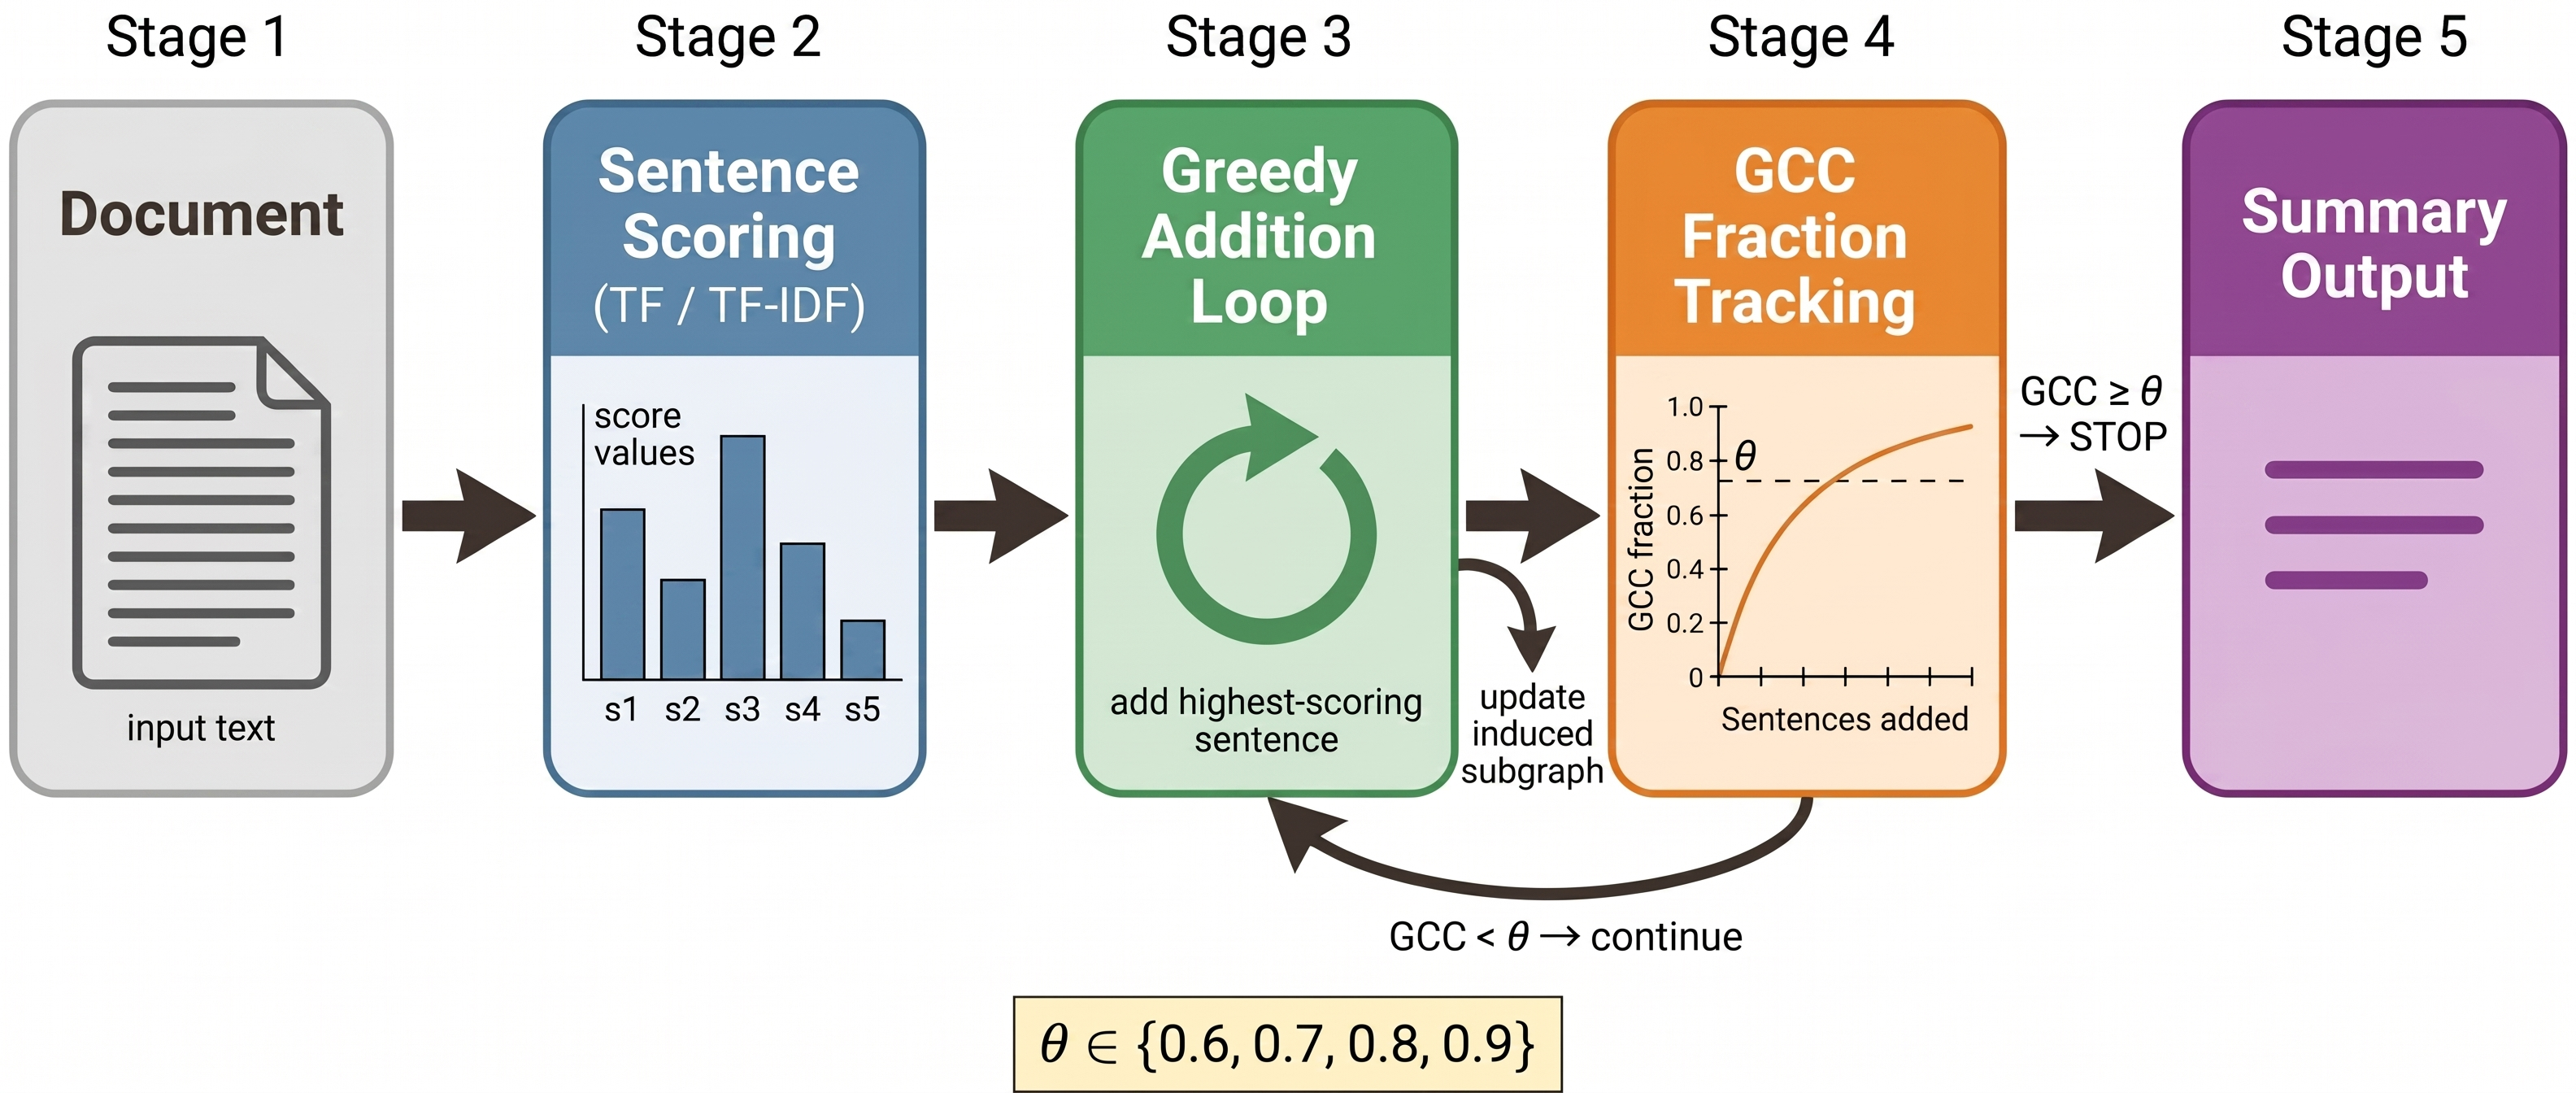
\includegraphics[width=\textwidth,height=0.45\textheight,keepaspectratio]{figures/fig_pipeline_v0.jpg}
  \caption{Overview of the percolation-threshold extractive summarization pipeline.
    A document's sentences are scored (TF or TF-IDF) and sorted. Sentences are added
    greedily; after each addition, the induced vocabulary co-occurrence subgraph is
    updated and its GCC size tracked. When the GCC fraction
    $\text{GCC}_{\text{summary}}/\text{GCC}_{\text{doc}}$ reaches threshold $\theta$,
    sentence selection stops. The result is a self-calibrating summary whose length is
    determined by the document's own vocabulary graph structure.}
  \label{fig:pipeline}
\end{figure*}

\paragraph{Summary of Contributions.}
(1) We introduce the first extractive summarizer using vocabulary co-occurrence graph
percolation as a self-calibrating stopping criterion, with a complete open-source
implementation (\S\ref{sec:methods}).
(2) We provide a rigorous evaluation on CNN/DailyMail ($n=2000$) and Multi-News
($n=1000$), comparing four percolation thresholds against three fixed-ratio baselines
with both TF and TF-IDF sentence scoring, with Holm-corrected Wilcoxon tests across all
pairwise comparisons (\S\ref{sec:experiments}).%
\footnote{Code: \url{https://github.com/AMGrobelnik/ai-invention-6a9498-vocabulary-percolation-threshold-for-sel/tree/main/round-2/experiment-1}}
(3) We report and analyze a structured negative finding: percolation maximizes recall but
not F1, and we identify the structural reasons---newswire vocabulary distribution in
CNN/DailyMail and the conciseness of all human reference summaries (\S\ref{sec:discussion}).
(4) We characterize how the percolation firing point varies across corpora
(\S\ref{sec:compression}), showing that Multi-News's multi-source vocabulary clustering
produces meaningfully different behavior from CNN/DailyMail's inverted-pyramid structure.
(5) We quantify that graph structural features explain only $R^2\approx 0.12$ of
compression variance, insufficient for reliable dynamic calibration
(\S\ref{sec:regression}).

\section{Related Work}

\paragraph{Extractive summarization.}
\citet{Luhn1958} introduced frequency-based sentence scoring. TextRank
\citep{Mihalcea2004} applies PageRank \citep{Page1999} over a sentence-similarity graph
and selects the top-$k$ sentences; LexRank \citep{Erkan2004} uses eigenvector centrality
over cosine-similarity sentences. Both require a fixed $k$. SummaRuNNer
\citep{Nallapati2017} uses a recurrent neural network to score sentences sequentially
with a fixed budget. BERTSum \citep{Liu2019bert} and PreSumm \citep{Liu2019presumm}
apply pretrained transformer encoders to sentence scoring. Neural abstractive methods,
including pointer-generator networks \citep{See2017}, similarly rely on externally
specified length constraints. None of these methods determines $k$ from the document's
intrinsic structure.

\citet{Ryang2012} use an influence propagation model on a word co-occurrence network to
maximize coverage under a budget constraint. The budget remains manually specified; the
phase transition is not used to determine when coverage is complete. Our work shares the
word-network foundation but replaces the manual budget with the percolation threshold.

\paragraph{Graph percolation in NLP.}
Erd{\H o}s--R\'enyi percolation theory \citep{ErdosRenyi1960,Bollobas2001} has been
applied to information diffusion in social networks and language evolution, but to our
knowledge has not previously been proposed as a stopping criterion for extractive
summarization.

\paragraph{CNN/DailyMail and Multi-News benchmarks.}
\citet{Hermann2015} introduced CNN/DailyMail for reading comprehension; it has since
become the standard single-document summarization benchmark \citep{See2017}. The
reference summaries are journalist-written bullet-point highlights (mean 42 words).
\citet{Fabbri2019} introduced Multi-News, a multi-document corpus aggregating 2--10 news
articles per story with a single reference summary. The multi-source structure gives
Multi-News stronger vocabulary segregation across its constituent documents, making it a
natural testbed for percolation-based stopping.

\section{Methods}
\label{sec:methods}

\subsection{Vocabulary Co-occurrence Graph Construction}%
\footnote{Code: \url{https://github.com/AMGrobelnik/ai-invention-6a9498-vocabulary-percolation-threshold-for-sel/tree/main/round-1/experiment-1}}

Given a document with sentences $s_1, \ldots, s_n$, we preprocess each sentence by
tokenizing, lowercasing, removing NLTK English stop words, and retaining alphabetic
tokens of length $\ge 2$. Let $W_i$ denote the content word set of sentence $s_i$.

The vocabulary co-occurrence graph $G = (V, E, w)$ is an undirected weighted graph.
Nodes $V$ are unique content words across the document. An edge $(u, v) \in E$ exists
between any two words $u, v \in W_i$ for some sentence $s_i$; the edge weight $w(u,v)$
equals the number of sentences in which $u$ and $v$ co-occur. The full-document GCC,
$\text{GCC}_{\text{doc}}$, is the node count of the largest connected component of $G$.

\subsection{Sentence Scoring}

We evaluate two sentence scoring functions. The \emph{TF scorer} ranks sentence $s_i$
by
\[
  \text{score}(s_i) = \sum_{w \in W_i} \text{TF}(w, D),
\]
where $\text{TF}(w,D)$ is the raw term frequency of word $w$ in document $D$. The
\emph{TF-IDF scorer} uses
\[
  \text{score}(s_i) = \sum_{w \in W_i} \text{TF}(w, s_i) \cdot \text{IDF}(w),
\]
treating each sentence as a sub-document and computing IDF over all sentences in the
document.

\subsection{Percolation-Threshold Stopping Criterion}

Given threshold $\theta \in (0,1)$, we add sentences greedily in descending score order.
After each addition, we update the \emph{induced subgraph} $G_S$ over accumulated
content words $\bigcup_{s_j \in S} W_j$ and compute $\text{GCC}_{\text{summary}}$ as
the largest connected component of $G_S$. The summary grows until:
\[
  \frac{\text{GCC}_{\text{summary}}}{\text{GCC}_{\text{doc}}} \geq \theta.
\]
If the ratio never reaches $\theta$, all sentences are retained. We evaluate $\theta \in
\{0.6, 0.7, 0.8, 0.9\}$, yielding eight percolation variants (2 scorers $\times$ 4
thresholds).

\subsection{Fixed-Ratio Baselines}

Baselines use the same sentence scoring and ordering as the percolation method. For ratio
$r \in \{0.10, 0.20, 0.30\}$, the summary consists of the top $\lceil r \cdot n \rceil$
sentences. This isolates the effect of the stopping criterion from sentence ranking.

\section{Experiments}
\label{sec:experiments}

\subsection{Datasets and Evaluation}

We use two corpora. \textbf{CNN/DailyMail 3.0.0} (2000 test documents; mean 575 words;
reference summaries mean 42 words, 2--5 sentences) \citep{Hermann2015}.
\textbf{Multi-News} test split (1000 documents; multi-source, one reference summary per
story) \citep{Fabbri2019}. Multi-News reference summaries are longer than CNN/DailyMail
highlights (approximately 250 words), reflecting the multi-source aggregation task. We
evaluate with ROUGE-1/2/L recall (R), precision (P), and F1 (F). Statistical
comparisons use two-sided Wilcoxon signed-rank tests with Holm--Bonferroni correction
over all pairwise comparisons.

\subsection{Main Results on CNN/DailyMail}

Table~\ref{tab:cnndm} reports mean ROUGE scores on CNN/DailyMail ($n=2000$). The results
expose a structural tension between recall and precision.

\begin{table}[!htbp]
  \centering
  \small
  \caption{Mean ROUGE scores on CNN/DailyMail ($n=2000$). CR = compression ratio
    (fraction of sentences selected). Bold indicates best ROUGE-1 F1 in each scorer
    category.}
  \label{tab:cnndm}
  \begin{tabular}{lrrrrr}
    \toprule
    Method & R-1 R & R-1 P & R-1 F1 & R-2 F1 & CR mean \\
    \midrule
    TF perc.\ $\theta{=}0.6$ & 0.772 & 0.112 & 0.187 & 0.092 & 0.597 \\
    TF perc.\ $\theta{=}0.7$ & 0.808 & 0.101 & 0.173 & 0.087 & 0.686 \\
    TF perc.\ $\theta{=}0.8$ & 0.834 & 0.092 & 0.161 & 0.084 & 0.773 \\
    TF perc.\ $\theta{=}0.9$ & 0.858 & 0.085 & 0.150 & 0.080 & 0.866 \\
    TF-IDF perc.\ $\theta{=}0.6$ & 0.743 & 0.126 & \textbf{0.205} & 0.092 & 0.369 \\
    TF-IDF perc.\ $\theta{=}0.7$ & 0.784 & 0.112 & 0.188 & 0.089 & 0.463 \\
    \midrule
    TF fixed@10\% & 0.296 & 0.313 & 0.274 & 0.092 & 0.100 \\
    TF fixed@20\% & 0.468 & 0.233 & \textbf{0.284} & 0.107 & 0.200 \\
    TF fixed@30\% & 0.578 & 0.183 & 0.259 & 0.107 & 0.300 \\
    \bottomrule
  \end{tabular}
\end{table}

\paragraph{Recall.}
At $\theta{=}0.9$, TF percolation achieves ROUGE-1 recall of 0.858 versus 0.578 for
fixed@30\% ($\Delta{=}{+}0.280$). All percolation variants significantly outperform all
fixed-ratio baselines on recall (Wilcoxon, all Holm-corrected $p<0.001$). Percolation
summaries contain more reference vocabulary because they include more sentences.

\paragraph{F1.}
Fixed-ratio summaries dominate on F1. TF fixed@20\% achieves ROUGE-1 F1$=0.284$, versus
0.205 for the best percolation variant (TF-IDF, $\theta{=}0.6$). The fixed baselines'
precision advantage more than compensates for lower recall. The best TF percolation
variant ($\theta{=}0.6$) achieves F1$=0.187$---34\% below the fixed@20\% F1.

\paragraph{Effect of TF-IDF scoring.}
TF-IDF selects fewer sentences than TF at the same $\theta$: CR mean of 0.369 vs.\ 0.597
at $\theta{=}0.6$, because TF-IDF up-weights document-specific rare words, which tend to
cluster in fewer sentences. This lower compression raises F1 to 0.205 for TF-IDF
percolation $\theta{=}0.6$, a 9.6\% absolute improvement over TF percolation at the same
$\theta$. However, it does not close the gap to fixed-ratio F1 (0.284): the scorer
interacts with the stopping criterion, but the stopping criterion remains the binding
constraint.

\paragraph{Ceiling fraction.}
For all percolation thresholds and scorers on CNN/DailyMail, the fraction of documents
where percolation selects all sentences is 0.0\%. The GCC ratio reaches every tested
$\theta$ value in every document, confirming that the sparse-graph edge case does not
arise in this corpus.

\begin{figure*}[!t]
  \centering
  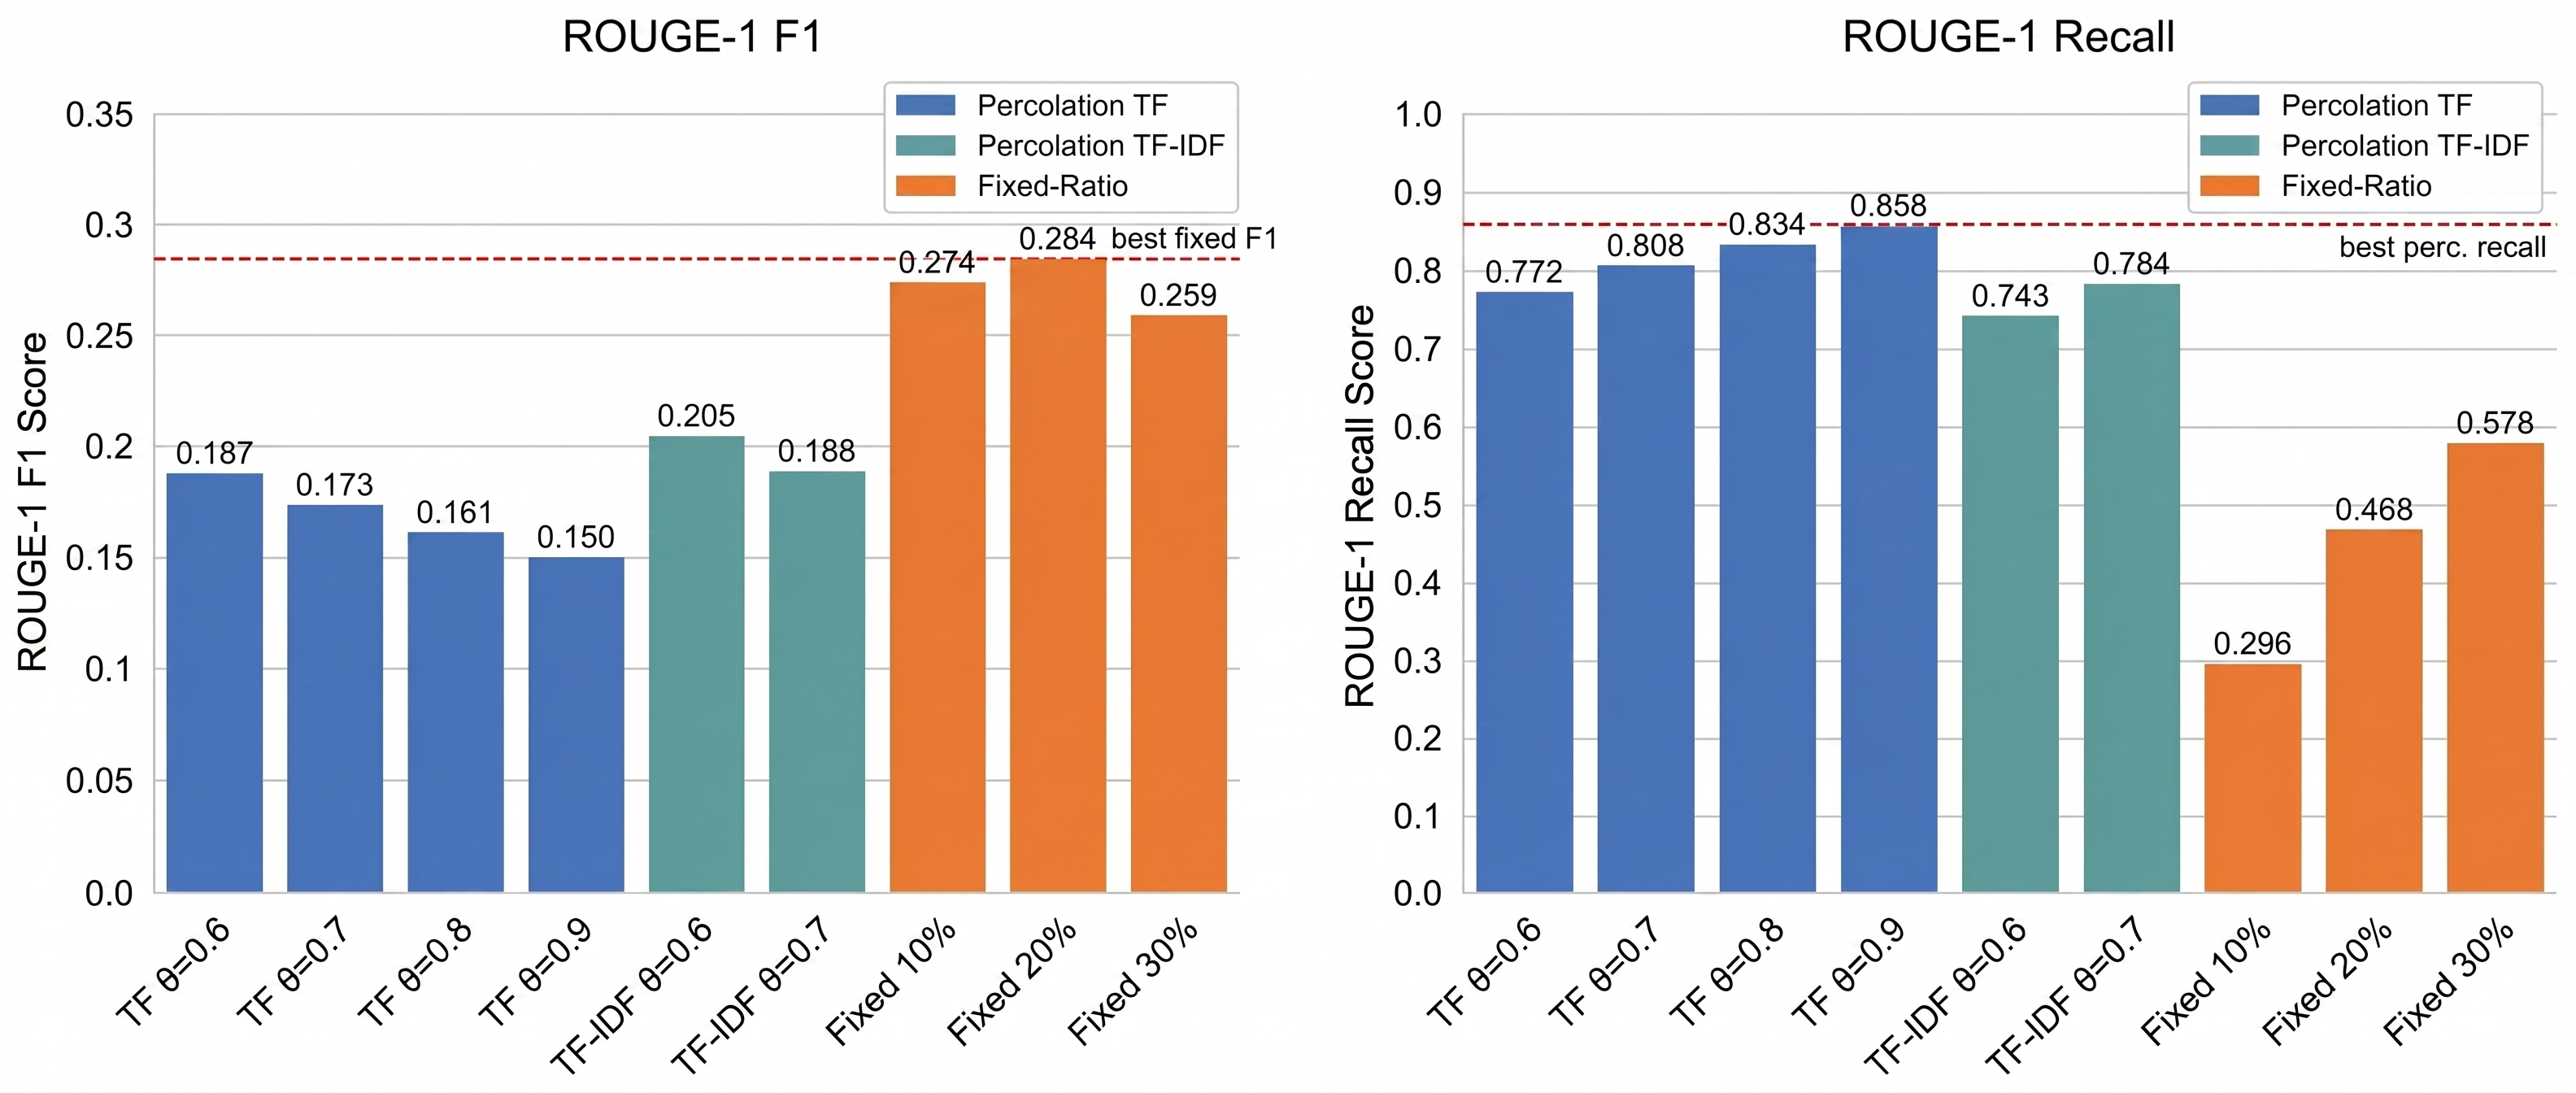
\includegraphics[width=\textwidth,height=0.45\textheight,keepaspectratio]{figures/fig_rouge_cnndm_v0.jpg}
  \caption{ROUGE-1 F1 (left panel) and ROUGE-1 Recall (right panel) for all evaluated
    methods on CNN/DailyMail ($n=2000$). Percolation variants (TF and TF-IDF,
    $\theta{=}0.6$--$0.9$) are shown in blue/teal; fixed-ratio baselines (TF,
    10\%/20\%/30\%) are shown in orange. Fixed-ratio baselines dominate on F1;
    percolation achieves substantially higher recall at the cost of lower precision.}
  \label{fig:rouge_cnndm}
\end{figure*}

\subsection{Multi-News Evaluation}

Table~\ref{tab:multinews} reports ROUGE-1 results on Multi-News (TF scorer;
$n=1000$).%
\footnote{Code: \url{https://github.com/AMGrobelnik/ai-invention-6a9498-vocabulary-percolation-threshold-for-sel/tree/main/round-2/evaluation-1}}

\begin{table}[!htbp]
  \centering
  \small
  \caption{Mean ROUGE-1 scores on Multi-News ($n=1000$, TF scorer). Fixed-ratio F1
    dominates, but percolation fires substantially earlier than on CNN/DailyMail.}
  \label{tab:multinews}
  \begin{tabular}{lrrrr}
    \toprule
    Method & R-1 R & R-1 F1 & CR mean & CR std \\
    \midrule
    TF perc.\ $\theta{=}0.6$ & 0.738 & 0.280 & 0.345 & 0.020 \\
    TF perc.\ $\theta{=}0.7$ & 0.770 & 0.253 & 0.457 & 0.046 \\
    TF perc.\ $\theta{=}0.8$ & 0.796 & 0.226 & 0.601 & 0.030 \\
    TF perc.\ $\theta{=}0.9$ & 0.817 & 0.207 & 0.742 & 0.019 \\
    \midrule
    TF fixed@10\% & 0.528 & \textbf{0.385} & 0.100 & --- \\
    TF fixed@20\% & 0.665 & 0.339 & 0.200 & --- \\
    TF fixed@30\% & 0.726 & 0.296 & 0.300 & --- \\
    \bottomrule
  \end{tabular}
\end{table}

Two findings distinguish Multi-News from CNN/DailyMail. First, percolation fires at a
meaningfully lower compression ratio: $\theta{=}0.6$ yields CR$=0.345$ on Multi-News
versus CR$=0.597$ on CNN/DailyMail. This supports the theoretical prediction that
documents with distinct vocabulary clusters (here, per-source articles merged into one
document) trigger the GCC criterion earlier, requiring fewer sentences to connect all
vocabulary communities. Second, the F1 gap between percolation and fixed-ratio baselines
narrows: the gap between percolation $\theta{=}0.6$ F1 and fixed@30\% F1 is 0.016 on
Multi-News (0.296$-$0.280) compared to 0.072 on CNN/DailyMail (0.259$-$0.187). The
percolation criterion is thus less mis-calibrated on Multi-News, but fixed ratios still
win.

\begin{figure*}[!t]
  \centering
  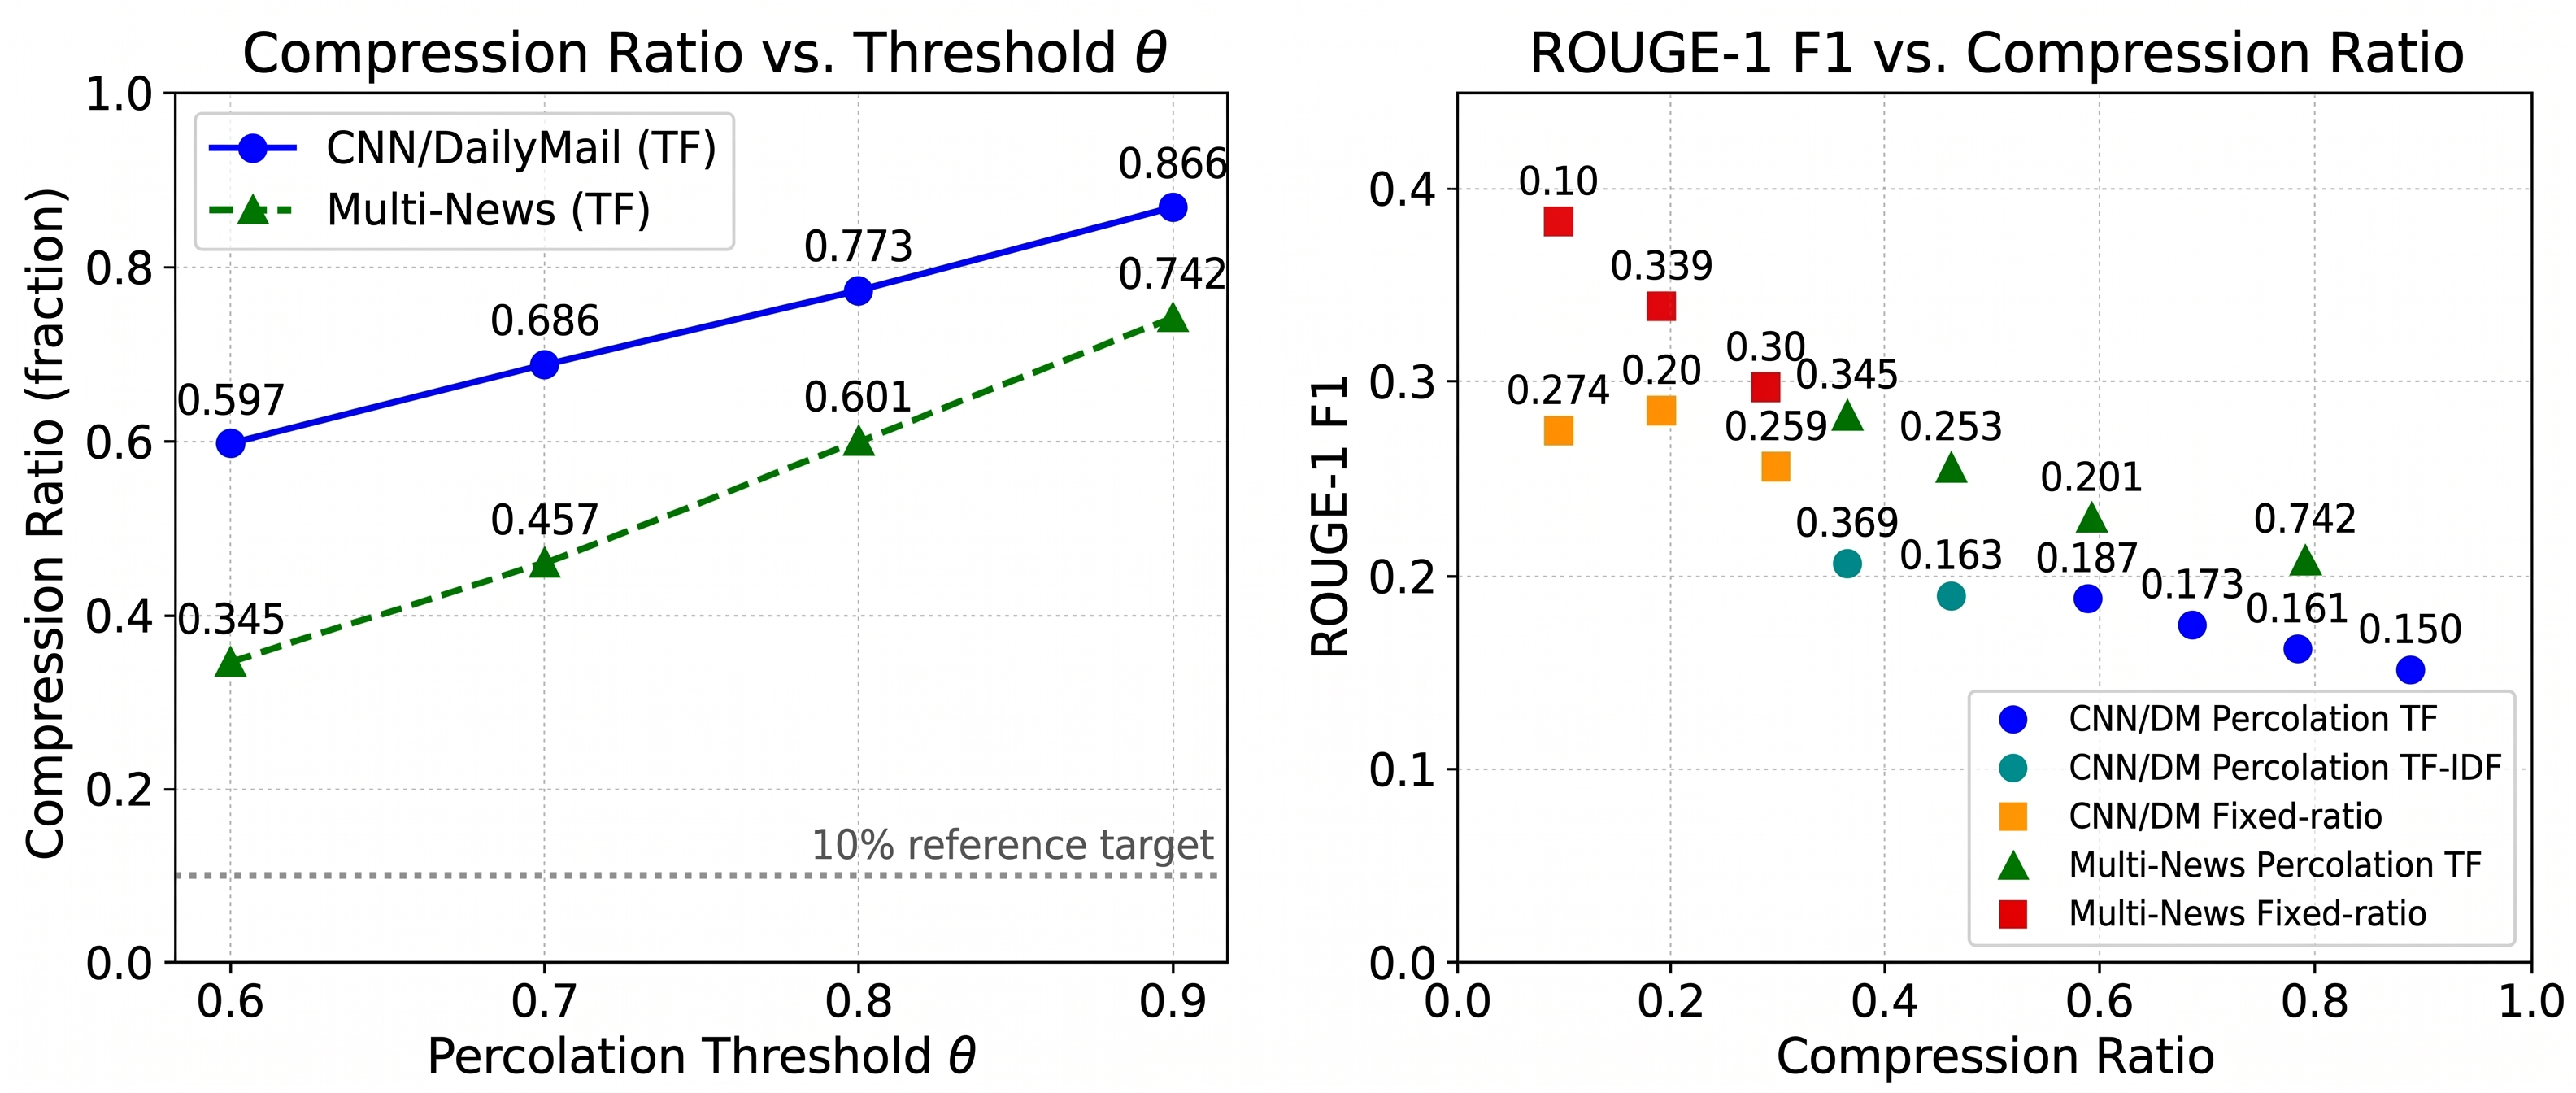
\includegraphics[width=\textwidth,height=0.45\textheight,keepaspectratio]{figures/fig_cross_corpus_v0.jpg}
  \caption{Left panel: Mean compression ratio (fraction of sentences selected) vs.\
    percolation threshold $\theta$ for CNN/DailyMail (blue) and Multi-News (green), TF
    scorer. Multi-News percolation fires at substantially lower compression ratios than
    CNN/DailyMail, reflecting stronger vocabulary clustering in multi-source documents.
    Right panel: ROUGE-1 F1 vs.\ compression ratio for all method-corpus combinations,
    showing that fixed-ratio baselines (orange squares for CNN/DM, red squares for
    Multi-News) dominate F1 at any given compression level.}
  \label{fig:cross_corpus}
\end{figure*}

\subsection{Compression Ratio Analysis}
\label{sec:compression}

Compression ratios on CNN/DailyMail cluster tightly: std$=0.075$--$0.077$ across TF
thresholds, and std$=0.083$--$0.086$ for TF-IDF. All standard deviations fall below the
10 percentage point discriminative threshold, indicating that the GCC fires at a
consistent fraction of document sentences regardless of article length or topic diversity
within this corpus. The interquartile range for TF $\theta{=}0.9$ spans approximately
81--93\% of sentences.

On Multi-News, the compression variance remains narrow at most thresholds
(std$=0.020$ at $\theta{=}0.6$ and 0.019 at $\theta{=}0.9$), with one exception at
$\theta{=}0.7$ (std$=0.046$). Neither corpus shows std $> 10$pp across most thresholds.
The variance finding does not support the theoretical prediction of document-adaptive
length selection.

Note that no tested $\theta$ produces mean compression near the 10\% target of reference
highlights on either corpus. The minimum mean compression is 34.5\% (Multi-News,
$\theta{=}0.6$) and 36.9\% (CNN/DailyMail, TF-IDF $\theta{=}0.6$). To match
reference-summary length ($\approx$10\% on CNN/DailyMail), a GCC fraction of
$\theta\ll 0.6$ would be required---a regime in which the GCC captures only a small
fraction of the document vocabulary and provides little coverage signal.

\subsection{Network Feature Regression}
\label{sec:regression}

Linear regression predicts the percolation compression ratio from five vocabulary graph
features: average degree, clustering coefficient, graph density, number of sentences, and
full GCC size. On CNN/DailyMail (TF scorer), $R^2=0.117$ at $\theta{=}0.6$, 0.127 at
$\theta{=}0.7$, and 0.134 at $\theta{=}0.8$, with graph density as the strongest
positive predictor (coefficient 0.546--0.596) and n\_sentences as the strongest negative
predictor (coefficient $-0.001$). The $R^2$ values indicate a statistically significant
but modest relationship: graph structure explains only 12--13\% of compression variance,
which is insufficient for reliable dynamic $\theta$ calibration. Proposed future
directions for dynamic calibration would need a substantially stronger predictor
($R^2\ge 0.5$) to outperform a fixed $\theta$ choice.

\section{Discussion}
\label{sec:discussion}

\subsection{Why Percolation Does Not Improve F1}

The core negative finding---confirmed on both CNN/DailyMail and Multi-News---is that
percolation-determined summaries are too long relative to human-written reference
summaries. CNN/DailyMail reference summaries span approximately 7--10\% of a typical
article; Multi-News references, while longer in absolute terms, remain concise relative
to the merged multi-source length. The percolation threshold correctly signals when the
vocabulary graph becomes \emph{connected enough}, but this connectivity criterion does
not correspond to the \emph{salience threshold} implicit in human-written highlights.

The mismatch is structural and not specific to TF scoring: replacing TF with TF-IDF
reduces compression ratios moderately but does not align percolation with the brevity of
reference summaries. TextRank and LexRank \citep{Mihalcea2004,Erkan2004} also require a
fixed $k$ and would face the same challenge: using percolation as their stopping
criterion would produce the same vocabulary-coverage-driven compression ratios.

The finding that no tested $\theta$ produces $\approx$10\% compression on CNN/DailyMail
reveals a deeper incompatibility: the percolation criterion requires a non-trivial
connected vocabulary structure, which cannot be achieved from 10\% of sentences in
typical newswire articles. A vocabulary graph sampled from 10\% of sentences is, in
almost all cases, highly disconnected---far below any reasonable GCC threshold. The
criterion is therefore structurally unable to produce short summaries on this corpus.

\subsection{Corpus-Conditional Behavior: A Theoretical Confirmation}

The cross-corpus comparison provides partial theoretical validation. Multi-News documents
aggregate articles on the same story from multiple sources; each source article introduces
source-specific vocabulary that forms a relatively isolated vocabulary cluster. Merging
2--10 source articles into one document creates a multi-cluster vocabulary graph in which
the GCC can be achieved by selecting a small number of inter-source bridging sentences.
This is precisely the vocabulary segregation scenario the hypothesis predicted would cause
the GCC to fire earlier---and indeed, $\theta{=}0.6$ fires at CR$=0.345$ on Multi-News
versus CR$=0.597$ on CNN/DailyMail.

However, even on Multi-News the compression variance remains narrow (std$\le 0.046$ at
all $\theta$ values). The within-corpus homogeneity reflects that all Multi-News documents
share the same multi-source aggregation structure, so the GCC fires at a structurally
consistent point. True document-adaptive compression would require a \emph{corpus-level
diversity} in document types---mixing single-topic and multi-topic documents---rather than
corpus-level homogeneity in one type.

\subsection{Implications for Percolation-Based Length Selection}

The results suggest three conditions under which a percolation stopping criterion could
be practically useful. First, the corpus should contain documents with diverse vocabulary
clustering structure (not homogeneous newswire or homogeneous multi-source). Second,
reference summaries should aim at coverage rather than concise highlights---scientific
review articles or technical documentation summaries, where completeness is valued over
brevity, may be better aligned with the GCC criterion. Third, the percolation criterion's
recall advantage ($+0.280$ on CNN/DailyMail at $\theta{=}0.9$) is directly useful for
retrieval or recall-oriented applications where missing content is more costly than
verbosity.

\subsection{Limitations}

\begin{itemize}
  \item \textit{Scorer coverage.} Only TF and TF-IDF scoring are implemented. TextRank
    and LexRank are discussed in Related Work but not evaluated as scorers. Sentence-level
    graph-based scorers may interact differently with the percolation stopping
    criterion---their graph structure partially overlaps with the vocabulary GCC,
    potentially creating complementary or interfering signals.

  \item \textit{$R^2=0.12$ is insufficient for dynamic calibration.} The regression
    analysis shows that graph structural features explain only 12--13\% of compression
    variance. Proposals to dynamically calibrate $\theta$ from graph features therefore
    cannot be expected to outperform a fixed $\theta$ choice; a much stronger feature
    representation ($R^2\ge 0.5$) would be needed.

  \item \textit{GCC definition.} The fraction $\theta$ is applied to the GCC node count.
    Alternative measures---edge density, spectral gap, modularity---may fire at different,
    more appropriate points. The GCC node fraction is one of several possible percolation
    signals.

  \item \textit{ER model caveat.} The classical Erd{\H o}s--R\'enyi percolation
    transition provides the motivating intuition for the method, but vocabulary
    co-occurrence graphs are not ER graphs: they have high clustering, heavy-tailed degree
    distributions, and community structure. The formal percolation threshold of an ER
    graph does not apply analytically, and $\theta$ must be treated as an empirical
    hyperparameter.
\end{itemize}

\section{Conclusion}

We proposed and evaluated the first extractive summarizer to use vocabulary co-occurrence
graph percolation as a self-calibrating length criterion. The method selects sentences
(by TF or TF-IDF score) until the summary's induced vocabulary subgraph forms a giant
connected component reaching fraction $\theta$ of the full document's GCC. On
CNN/DailyMail ($n=2000$), percolation at $\theta{=}0.9$ achieves ROUGE-1 recall of
0.858 versus 0.578 for the best fixed-ratio baseline, while fixed@20\% dominates on F1
(0.284 vs.\ 0.205 for the best percolation variant). On Multi-News ($n=1000$), percolation
fires substantially earlier (CR$=0.345$ at $\theta{=}0.6$ vs.\ CR$=0.597$ on
CNN/DailyMail), confirming the theoretical prediction about vocabulary segregation in
multi-source documents---yet fixed-ratio F1 still dominates (fixed@10\%: 0.385 vs.\
percolation $\theta{=}0.6$: 0.280). The failure mode is structural: the GCC criterion
targets coverage completeness, whereas human-written highlights target salience and
brevity. Network features explain only $R^2\approx 0.12$ of compression variance, ruling
out reliable dynamic calibration from graph topology alone.

Future work should evaluate the percolation criterion on corpora that combine documents
of diverse vocabulary clustering---multi-topic review articles or heterogeneous
collections that mix focused and broad documents within a single evaluation set---where
the criterion may provide document-adaptive compression rather than corpus-level
homogeneous compression. Replacing the GCC node count with richer percolation signals
(spectral gap, modularity) and applying the criterion to recall-oriented retrieval
settings rather than F1-optimized summarization may also yield settings where the
percolation criterion's coverage-maximizing behavior is directly beneficial.

\bibliographystyle{plainnat}
\bibliography{references}

\end{document}
